\section{\textsc {Task \uppercase\expandafter{\romannumeral1}}: Dynamic SHG( \underline{S}equestering-\underline{H}arvesting-\underline{G}rowing) Simulation Model}
\subsection{Model Overview}
To better use the resources in the forest, the schedule of forest managing will contain the timber harvesting processes of tree cutting. After harvesting the log from the wood, the log will be made into different kinds of wood products. And apart from generating economic value, the harvesting activities will also speed up the carbon sequestering process.

To quantify the carbon sequestered by the forest, we categorize the amount of the total carbon sequestration ($TCS$) into three sections, which come from the mature forest area ($CS_{ma}$), the growing forest area ($CS_{gr}$), and the product produced from the log in the forest($CS_{pr}$). 

\begin{equation}
   TCS = CS_{ma} + CS_{pr} + CS_{gr} \label{XX}
\end{equation}

The dynamic process of sequestering, harvesting and growing is shown in Fig. [\ref{Dynamic process of sequestering}]. After the categorization, we will give the definitions of the three parts.

\begin{figure}[H]
\centering
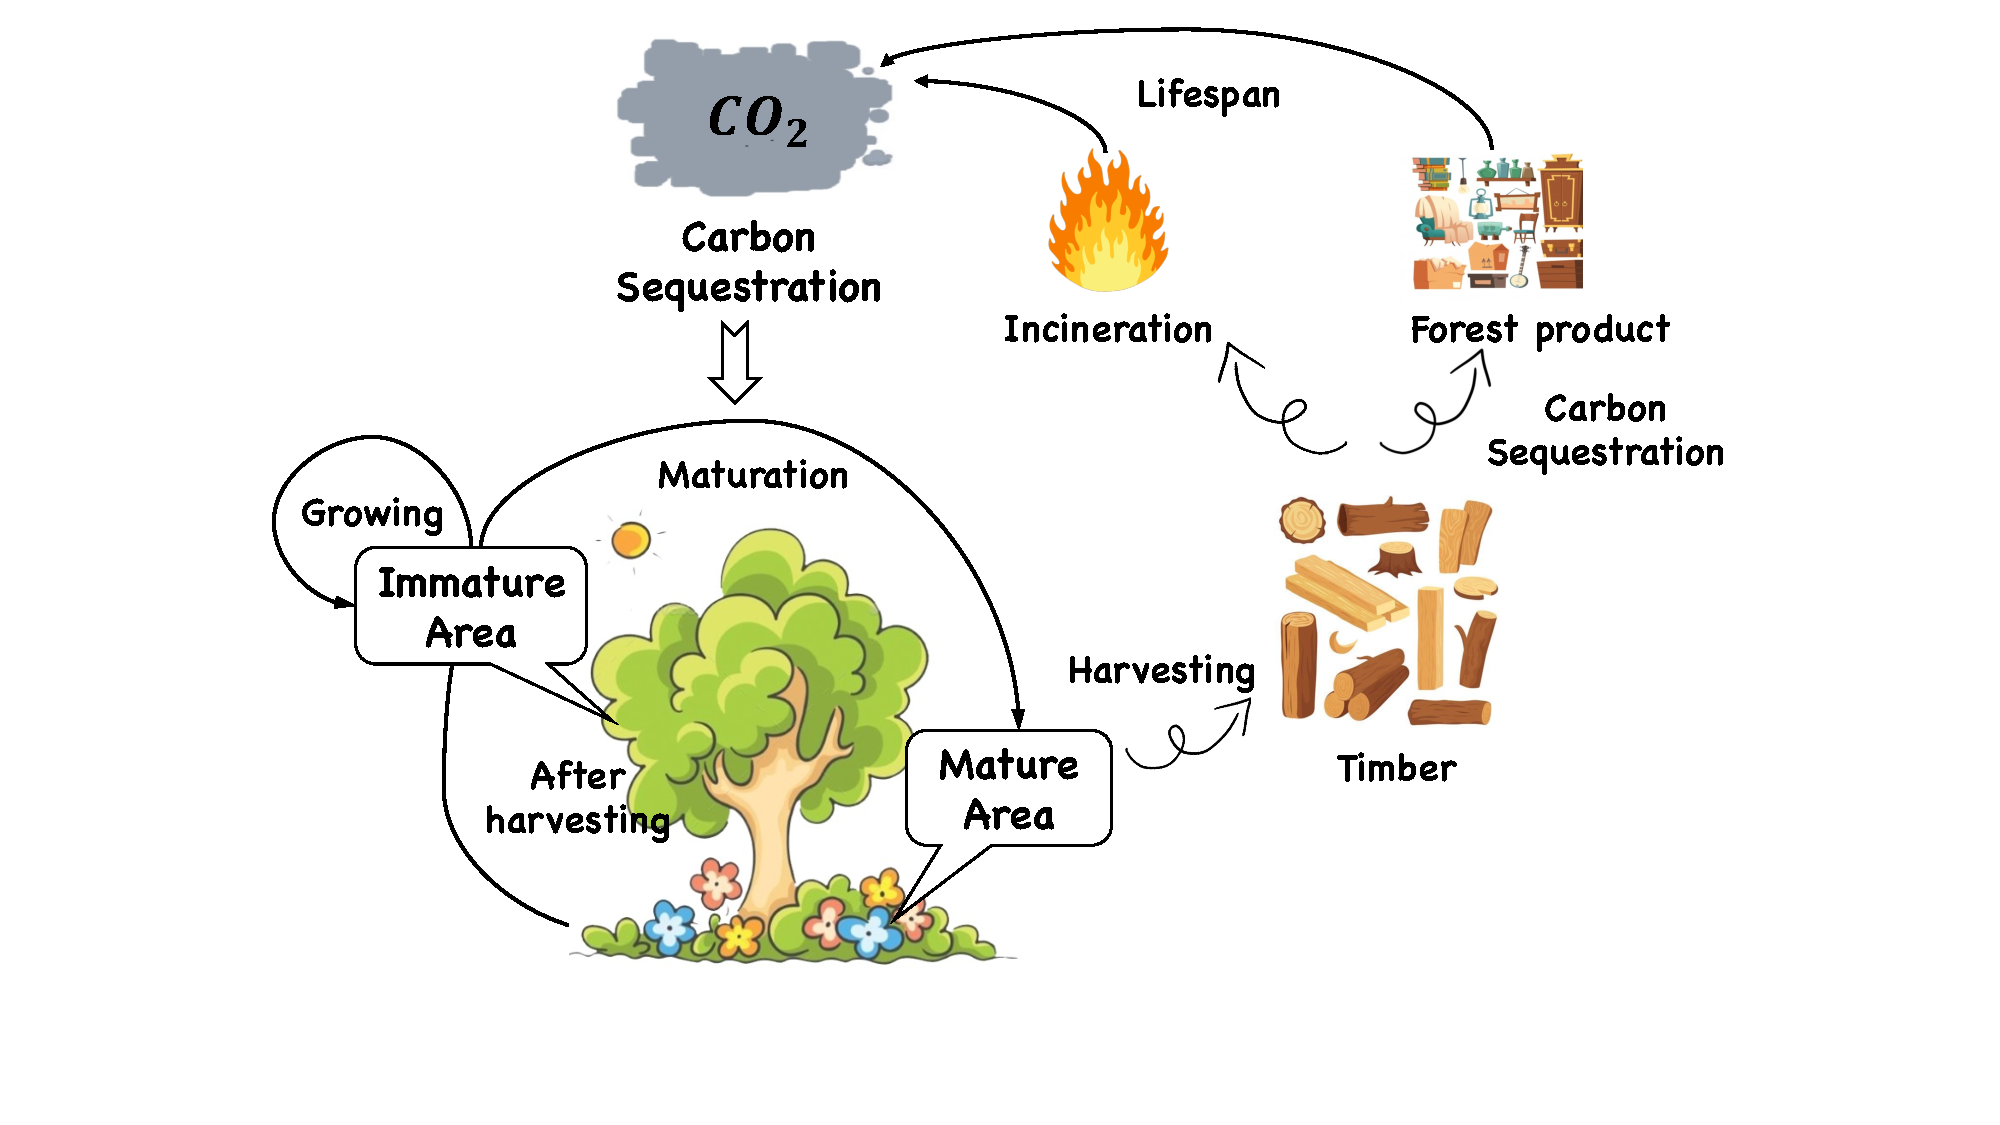
\includegraphics[scale = 0.4]{mcmthesis-demo/figures/Dynamic Process of Carbon Cycle .pdf}
\caption{Dynamic process of sequestering, harvesting and growing} 
\label{Dynamic process of sequestering}
\end{figure}

\subsection{Dynamic Carbon Cycle Simulation}
\subsubsection{Sequestering: The Mature Area}
Forest is the central part of the global carbon cycle. During its growth, land plants in the forest can synthesize organic matter by absorbing $CO_2$ within a specific concentration range, thus saving the cost of carbon sequestration by some technologies like separation and purification. 

Because the annual carbon conversion rate of different types of trees per square hectare can be obtained in previous studies, the carbon sequestration stock of mature forest can be calculated directly by using the following formula where the $\Delta T$ is the period of time. 
For $v_{t,i}$ may varies in different years, we use summation sign to express the accumulation in $\Delta T$, the same as below.
\begin{equation}
S_{ma} = S-\sum_{growing}S_{area}+\sum_{\substack{finish \\ growing}}S_{area}
\end{equation}
\begin{equation}
CS_{ma} = S_{ma}\sum_{t=1}^{\Delta T}v_{t,i}
\end{equation}

The expression shows the mature part's area is dynamic annually in our model, for we've considered the growing process of the previously harvested area. When the growing process is completed, the land will be recalculated as a part of the mature area.

\begin{comment}
\begin{figure}[H]
\centering
\includegraphics[scale = 0.25]{mcmthesis-demo/figures/area.png}
\caption{Global forest area by country, 2020 \cite{area}} 
\end{figure}
\end{comment}

\subsubsection{Harvesting: The Forest Products}
Harvested trees can be used for various purposes, including wood fuel, industrial roundwood, plywood, paper, and more. Among these, the carbon in wood fuel is incinerated and returns to the atmosphere. 
This process cannot be classified as carbon sequestration so we define the lifetime of wood fuel is 0. On the contrary, other forest products can complete carbon sequestration during their lifespan and return to nature as inorganic carbon once their lifespan ends. The lifespans of forest products are shown in Tab. [\ref{table3}].

\begin{table}[h]
	\centering
%   \vspace*{-14cm}              % 调整图像上间距
	\caption{Average lifespan of different forest products \cite{article}}
	\tabulinesep=1mm
	\begin{tabu}to \linewidth{X[c,m]X[2.5,c,m]X[c,m]}
		\tabucline[0.08em]-
		$i$ & $Item$                                  & $als_i$  \\ \tabucline[0.08em]-
		1	& Industrial roundwood                    & 15.3     \\
		2	& Wood pellets and other agglomerates     & 4.1	     \\
		3	& Sawnwood                                & 21.0	 \\
		4	& Wood-based panel                        & 7.5	     \\
		5	& Papers                                  & 29.8     \\
		\tabucline[0.08em]-
	\end{tabu}
%   \vspace*{-5mm}              % 调整图像下间距
    \label{table3}
\end{table}

We assume that the carbon sequestrated in product i released at a constant speed and the forest products structure in the specific region is stable. When region j is determined, the formula below can give the carbon sequestration of products. $pp_{i,j}$ denotes the product i's ratio of all the wood product in region j. The data of $pp_{i,j}$ can be obtained in Brunet-Navarro et al, 2017\cite{article}.
\begin{equation}
CS_{pr} = \sum_{t=1}^{\Delta T}S\alpha\omega\sum\limits _{i=1}^{5} \frac{pp_{i,j}}{als_i}
\end{equation}

% \begin{figure}[H]
% \centering
% \includegraphics[scale = 0.2]{mcmthesis-demo/figures/product1.png}
% \caption{Forest products structure of 6 continents} 
% \end{figure}

\subsubsection{Growing: The Growing Area}
In this part, we will give the definition of the amount of carbon that sequestrated by the growing area of the forest.

For the trees in a particular area in the forest, the growth rate for the trees will gradually slow down as the maturity of this block of forest increases. By now, the tree will not have sufficient space to grow any further. 
And if the land is completely wiped out, the process for the bare ground transforming into the forest will be extremely long, and to fully restore may take over a century\cite{1}. 
So, drawing the inspiration from  Pierre-Franois Verhulst's mathematical model, we formulate the growing area $i$'s full rate $fr_{area,i}$ in total using the logistic model to calculate the initial time $t_{ini}$ after one area's harvest.

\begin{equation}
    \frac{dfr_{area, i}}{dt} = C_0fr_{area, i}(1-\frac{fr_{area, i}}{1})
\end{equation}

In the logistic model, $C_0$ is called the growth rate, which negatively correlates to $c_i$. $i$ refers to different types of forest or trees and $S_{area}$ denotes the area of the harvested land $i$. For this model, when $t = \frac{c_i}{2}$, the $fr_{area, i}$ will equal to 0.5. So $t$ can be expressed as:

\begin{equation}
    fr_{area, i}(t) = \frac{1}{e^{-\frac{C_0t}{c_i} + \frac{C_0}{2}}+1} \label{N_i}
\end{equation}

According to different types of forests, $C_0$ may be different. Considering the time, we expect that when $t = c_i$, the $fr_{area, i}$ will reach approximately 1. So we give that:

\begin{equation}
    fr_{area, i}(c_i) = \frac{1}{e^{-\frac{C_0}{2}}+1} \geq 0.95
    \Rightarrow
    C_0 \geq 2ln19 = 5.88
\end{equation}

After harvesting, the mature area becomes an immature area, and the corresponding growth time $t_{ini}$ can be calculated via $fr_{area, i}$. In the formula, we round down $t_{ini}$ to simplify the calculation.

\begin{equation}
    fr_{area, i} = \frac{1}{e^{-\frac{8t_{ini}}{c_i} + 4}+1} \\\\
    \rightarrow
    t_{ini} = \Bigl\lfloor \frac{c_i}{C_0}(ln(\frac{fr_{area, i}}{1-fr_{area, i}}) + \frac{C_0}{2}) \Bigr\rfloor
\end{equation}

As the tree continues to grow, the area's density is getting closer to saturated status, so the pace of growth is slowing in the meantime. As Fig. [\ref{fig:waixian}] from the FAO shows that the speed of carbon sequestrating rises rapidly and felling down slowly with the bare area as the initial state.

\begin{figure}[h]
    \centering
    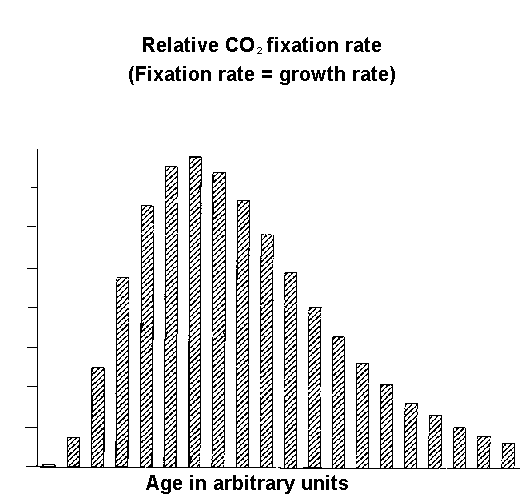
\includegraphics[scale = 0.35]{mcmthesis-demo/4/image.png}
    \caption{Typical carbon dioxide fixation rate of a tree as a function of its age\cite{2}}
    \label{fig:waixian}
\end{figure}

To simplify the model, we use logarithmic functions to construct expressions $v_{i}'(t)$ to fit data above in the shape of skewed distributions.

\begin{equation}
    v_{i}'(t) = q_i\frac{ln(p_it+1)}{p_it+1}
\end{equation}

Where $p_i$ and $q_i$ denote two coefficients of different forests or trees. 
By adjusting these two coefficients, the curve can change into various shapes, which can fit the discrete data in Fig. [\ref{fig:waixian}].
\begin{figure}
    \centering
        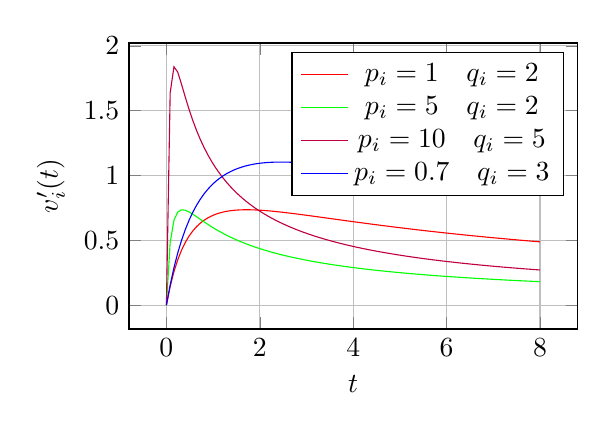
\begin{tikzpicture}
            \begin{axis}[domain=-0:8,samples=100,grid=major,width = 0.6\linewidth,height = 0.43\linewidth,
                restrict y to domain=0:4,xlabel=$t$,ylabel=$v_{i}'(t)$, legend pos=north east]
            \addplot [color=red]    {2*(ln(x+1))/(x+1)};
            \addplot [color=green]  {2*(ln(5*x+1))/(5*x+1)};
            \addplot [color=purple] {5*(ln(10*x+1))/(10*x+1)};
            \addplot [color=blue]   {3*(ln(0.7*x+1))/(0.7*x+1)};
            
           \legend{$p_i = 1\quad q_i = 2$, $p_i = 5\quad q_i = 2$, $p_i = 10\quad q_i = 5$, $p_i = 0.7\quad q_i = 3$}/
            \end{axis}
        \end{tikzpicture}
        \vspace{-1ex}
    \caption{Speed fitting curve with different $p_i$ and $q_i$}
    \label{fig:my_label}
\end{figure}

Charlotte E. Wheeler et al. \cite{3} find that the biomass accumulation increased fourfold to 3.9 Mg $\text{ha}^{-1} \text{y}^{-1}$ between 10 and 18 years.
And two graphs in Kotaro Iizuka's research \cite{4} also show that the highest rate of carbon sequestration of coniferous forest, deciduous broadleaf forest and evergreen broadleaf forest all occur in the group of 15-20 years, whose results are consistent with FAO's graph of Fig [\ref{fig:waixian}].

We can figure out that when $t = \frac{e-1}{b}$, $v_{i}'(t)$ will reach its maximum level $\frac{a}{e}$. So, we can define that:

\begin{equation}
\left\{
    \begin{aligned}
        &\frac{e-1}{p_i} = t_{i, max} \\ &\frac{q_i}{e} = v_{i, max}
    \end{aligned}
\right.    
\Rightarrow
\left\{
    \begin{aligned}
        &p_i = \frac{e-1}{t_{i, max}} \\ &q_i = ev_{i, max}
    \end{aligned}
\right.    
\end{equation}

Where $v_{i, max}$ denotes the max carbon sequestrating speed of different kinds of forests or trees, $t_{i, max}$ denotes the age of reaching $v_{i, max}$. Based on the data of Kotaro Iizuka, et al.\cite{4}, Meenakshi Kaul, et al.\cite{5}, the carbon sequestrating speed calculating sheet are as follows:

\begin{table}[h]
	\centering
%   \vspace*{-14cm}              % 调整图像上间距
	\caption{Carbon sequestrating speed calculating sheet}
	\tabulinesep=1.1mm
	\begin{tabu}to \linewidth{X[c,m]X[2.5,c,m]X[c,m]X[c,m]X[c,m]X[c,m]}
		\tabucline[0.08em]-
		$i$ & $tree / forest\ type$          & $p_i$     & $q_i$     & $v_{i, max}$  & $t_{i, max}$\\\tabucline[0.08em]-
		1	& Eucalyptus                    & 0.430     & 72.034    & 26.5 	        & 4\\
		2	& Poplar                        & 0.430	    & 75.242 	& 27.68 	    & 4\\
		3	& Sal                           & 0.022	    & 26.367 	& 9.7 	        & 75\\
		4	& Teak                          & 0.115	    & 28.542 	& 10.5 	        & 15\\
		5	& Coniferous                    & 0.115     & 43.792 	& 16.11 	    & 15\\
		6	& Deciduous Broadleaf           & 0.115     & 18.729 	& 6.89 	        & 15\\
		7	& Evergreen Broadleaf           & 0.115     & 18.83     & 6.93 	        & 15\\
		\tabucline[0.08em]-
	\end{tabu}
%   \vspace*{-5mm}              % 调整图像下间距
    \label{table}
\end{table}

After finishing $v_{i}'(t)$ speed function, we can now give the definition of $CS_{gr}$. It reflects the amount of the carbon sequestrated by the growing area in the time period $\Delta T$ after the harvesting process of rate $\alpha$.

\begin{equation}
    \begin{aligned}
            CS_{gr} &= \sum_{area}\sum_{t = t_{ini}}^{t_{ini} + \Delta T} {S_{area, i} v_{area_i}}
                    &= \sum_{area}\sum_{t = t_{ini}}^{t_{ini} + \Delta T} \alpha\beta S v_{area,i}
    \end{aligned}
\end{equation}

Here, $v_{area,i}$ is the speed of carbon sequestrating of one growing area of forest kind $i$, which can be calculated through Tab. [\ref{table3}].

\subsection{Results}
To conclude our model by adding three parts up, the amount of carbon sequestrating of a year can be calculated as follow:

\begin{equation}
    \begin{aligned}
       TCS  &= CS_{ma} + CS_{pr} + CS_{gr}\\
            &= (S-\sum_{growing}S_{area}+\sum_{\substack{finish \\ growing}}S_{area})\sum_{t=1}^{\Delta T}v_{t,i}
            + \sum_{t=1}^{\Delta T}S\alpha\omega\sum\limits _{i=1}^{5} \frac{pp_{i,j}}{als_i}
            + \sum_{area}\sum_{t = t_{ini}}^{t_{ini} + \Delta T} \alpha\beta S v_{area,i}
    \end{aligned}
    \label{model}
\end{equation}
\subsubsection{Reaching the maximum of carbon sequestration with fixed $\alpha$} \label{Reaching}
Using the model in equation (\ref{model}), we can measure the total carbon sequestration of the forest. 
In this section, we use related data of evergreen broadleaf forests to test our model in a relatively short period of time. Given that the duration is short, we assume that all the data above will retain, and we will use the different time period to test the given forest model. 
Retrieved from FAO's website \cite{7} and l’IGN \cite{8}, the related figure and parameters are as follows:

\begin{table}[h]
	\centering
%   \vspace*{-14cm}              % 调整图像上间距
	\caption{Related parameters of evergreen broad-leaf forests}
	\tabulinesep=1mm
	\begin{tabu}to \linewidth{X[0.9,c,m]X[1.2,c,m]X[3,c,m]}
		\tabucline[0.08em]-
		variables           & values                        & function          \\\tabucline[0.08em]-
		$S$	                & 5000 ha                       & The total forset area of this case              \\
		$c_{eb}$	        & 50 year                       & The average life span of the trees  \\
		$v_{t, eb}$	        & 5.3 tonne/year$\cdot$ha         & The carbon sequestration rate of the mature area 	            \\
		$\rho_{eb}$	        & 0.54 tonne/m^3                & The average density of the live wood \\
		$\omega_{eb}$	    & 112m^3/ha                     & the average growing stock    \\
		$C_0$               &8                              & The coefficient used to express $t_ini$\\
		$p_{eb}$	        & 0.115                         & \multirow{2}{*}{\begin{tabu}[r]{@{}X[c,m]@{}}Two coefficient used to calculate the restoration rate of the growing part \end{tabu}}\\
		$q_{eb}$	        & 18.83                         &\\
		\tabucline[0.08em]-
	\end{tabu}
%   \vspace*{-5mm}              % 调整图像下间距
    \label{table4}
\end{table}

We run our model under period of 5 years and 15 years, and we set $\beta \in [1,10]$, and $\alpha \in (0,1)$, and use Monte Carlo method $10 ^ 4$ times per test.
Setting the maximum carbon sequestration of the target, in the 5-year model, the result gives that when $\alpha = 0.0770$ and $\beta = 2.62$, the maximum level of carbon sequestration in total will be 139523.604 tonne in 5 years.
And in the 15-year model, the simulation shows that when $\alpha = 0.0381$ and $\beta = 5.73$, the maximum level of carbon sequestration in total will be 415367.965 tonne in 15 years.

When just considering a very short period of time, the best harvest rate is around 8\% of the total living stock of the forest, and $\beta = 2.62$ points out that harvest activities must be concentrated into a smaller area in order not to damage the large mature area. And when considering the longer period, the model's result shows that the best harvest rate is around 3.8\% of the total living stock of the forest, and $\beta = 5.73$ points out that harvest activities must be separated into a larger area of 5.7 times rather than totally wiping out a tiny amount of area. The instruction given by this model is consistent with the universal knowledge of distributed harvesting. 

\begin{figure}[h]
    \centering
        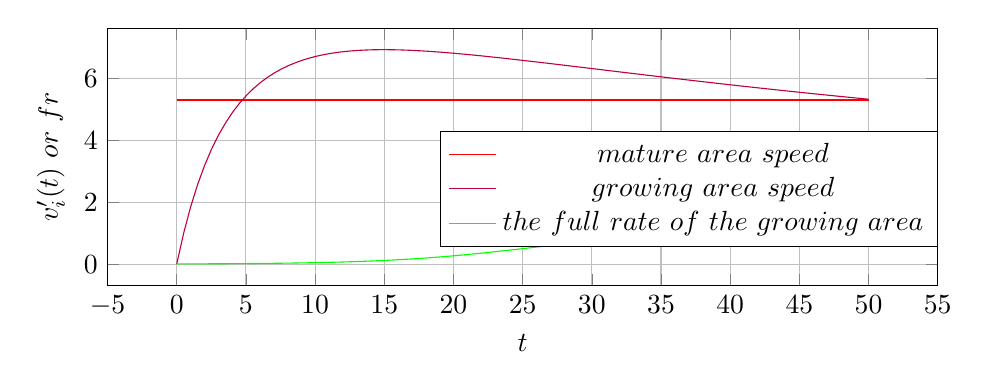
\begin{tikzpicture}
            \begin{axis}[domain=-0:50,samples=100,grid=major,width = \linewidth,height = 0.4\linewidth,
                restrict y to domain=0:8,xlabel=$t$,ylabel=$v_{i}'(t)\ \text{or}\ fr$, legend style={at={(1,0.6)}}]
            \addplot [color=red]    {5.3};
            \addplot [color=purple] {18.83 * (ln(0.115*x+1))/(0.115*x+1)};
            \addplot [color=green]  {1 / (1 + e^(5 - 0.2 * x))};
            
            
           \legend{$mature\ area\ speed$, $growing\ area\ speed$, $the\ full\ rate\ of\ the\ growing\ area$}/
            \end{axis}
        \end{tikzpicture}
    \vspace{-1.5ex}
    \caption{Curves used in the test}
    \label{Curves used in the test}
\end{figure}

\subsubsection{Reaching the maximum of carbon sequestration with dynamic $\alpha$}

Last test, we made the proportion of tree harvest $\alpha$ to be fixed in during the test. 
But in the reality, our managers have to adjust the coefficient $\alpha$ to change the total amount of harvesting logs. 
One effective way of adjusting $\alpha$ is using the negative feedback mode. 
When the total amount of wood in the forest is decreasing compared to the last year, the manager will lower $\alpha$ to reduce the log production activities this year to restore the level of ecology. 
And after the restoration, the total amount of wood in the forest will return to the higher level. So the manager can adjust $\alpha$ higher to increase the timber production. 
In a long time, the forest will reach a stable fluctuating state.

The definition of how $\alpha$ change chronologically is listed as the formula below.

\begin{equation}
    \alpha_{this\ year} = \alpha_{last\ year} \times \frac{TA_{last\ year} - Sw\rho \alpha_{last\ year} + CS_{gr, last\ year}}{TA_{last\ year}}
\end{equation}

Where $TA_i$ denotes the total amount of wood in the forest in year $i$.

We apply this method in the forest model in section \ref{Reaching}. From the result, we can plot the changes of $\alpha$ and the $TCS$ thorough 15 years of the simulation. The results shows that the initial $\alpha = 0.0407$, and it begins to fall to about 0.38. Then as the immature area sequesters faster than the mature area, the $TCS$ ratio begin to rise, so does the $\alpha$. Finally, the $TCS$ is higher than the one under the fixed $\alpha$ by 5\textperthousand. Meanwhile, $\alpha$ can finally rise to around 0.05, meaning more logs can be produced in this forest than the fixed $\alpha$ situation. 

\begin{figure}[h]
  \centering
  \hspace{-4.5cm}
  \begin{minipage}[b]{0.32\textwidth}
        \begin{tikzpicture} %tikz图片
            \begin{axis}[
                xlabel=year, %横坐标名
                ylabel=TCS ratio, %纵坐标名
                tick align=outside, %刻度在外显式
                legend style={at={(0,-0.2)},anchor=north} %图例在图下方显示
                ]
            \addplot[smooth,mark=*,blue] plot coordinates { 
                ($2^10$ ,0.0067)
                ($2^11$ ,0.1060)
                ($2^12$ ,0.1120)
                ($2^13$ ,0.1470)
                ($2^14$ ,0.2430)
                ($2^15$ ,0.3790)
                ($2^16$ ,0.7540)
                ($2^17$ ,1.4760)
                ($2^18$ ,2.9600)
                ($2^19$ ,6.0020)
                ($2^20$ ,12.182)
                ($2^21$ ,24.840)              
                % ($2^22$ ,1.000242669)
                % ($2^23$ ,1.000440004)
                % ($2^24$ ,1.000635594)
                % ($2^25$ ,1.000635594)
                % ($2^26$ ,1.000635594)
                % ($2^27$ ,1.000635594)
                % ($2^28$ ,1.000635594)
                

            };
            \end{axis}
        \end{tikzpicture}
  \end{minipage}
\hspace{3cm}
  \begin{minipage}[b]{0.32\textwidth}
    	\begin{tikzpicture} %tikz图片
            \begin{axis}[
                xlabel=year, %横坐标名
                ylabel=$\alpha$, %纵坐标名
                tick align=outside, %刻度在外显式
                legend style={at={(0.3,-0.2)},anchor=north} %图例在图下方显示
                ]
            %第一条线,mark是折线标示形状
            \addplot[smooth,mark=*,blue] plot coordinates { 
                (1,0.040737644)
                (2,0.039078089)
                (3,0.038246429)
                (4,0.038375118)
                (5,0.039287498)
                (6,0.040879699)
                (7,0.041908266)
                (8,0.042755375)
                (9,0.043653347)
                (10,0.044745594)
                (11,0.045843713)
                (12,0.046901650)
                (13,0.047944652)
                (14,0.049027589)
                (15,0.050140324)

            };
            \end{axis}
        \end{tikzpicture}
  \end{minipage}
  \hspace{-1cm}
  \caption{Left: TCS ratio of dynamic and fixed $\alpha$\quad Right: Dynamic change of $\alpha$ in 15 years}
\end{figure}